\section{Introduction}

Over the last decade global interest in wave energy has grown considerably, with
the Ocean Energy Systems executive committee setting a goal of 300GW of
installed ocean energy capacity by 2050
\citep[]{huckerbyInternationalVisionOcean2017}. This has been driven by concerns
about greenhouse-gas driven climate change, carbon-based energy price
volatility, and a growing emphasis on the value of diversifying energy
sources. Wave energy is seen as particularly valuable for its predictability and
reliability on timescales of hours to a few days
\citep{parkinsonIntegratingOceanWave2015}, and for the fact that the resource is
concentrated along coastlines where large fractions of the world's populations
live. Wave energy technology is still at an early-stage of technology
development with a wide-range of device archetypes under active development
\citep[]{babaritOceanWaveEnergy2017}.

During these early years of wave energy research and development, it has been
important to quantify the wave energy resource so that decision makers can begin to understand the market opportunity of this new technology. This has led to a
proliferation of publications on wave resource assessment. However, the
methods and results in these works are not always consistent, which can lead to confusion and skepticism. In this context the international electrotechnical commissions's technical committee on marine energy (IEC TC114) has been working to clarify the terminology and methods for describing and quantifying marine energy opportunities. This task is complicated by the need to quantify the opportunity at multiple scales (from the scale of a single project or device, all the way up to regional and national assessments), and a need to consider technical and practical constraints on the opportunity. To clarify this space, IEC TC114 has defined three types of resource assessment
\citep{internationalelectrotechnicalcommissionPartTerminology2011} \note{These
definitions are the ED2 defs, but this citation is the original. Need to update
once Ed-2 is published. Also: how do these definitions compare to what is used
for RA of wind/solar? Is that important?}:

\begin{itemize}
  \item the { \it theoretical resource} is the ``energy available in the resource''
  \item the {\it technical resource} is the ``proportion of the theoretical resource that can be captured using existing technology options without consideration of external constraints''
  \item the {\it practical resource} is the ``proportion of the technical resource that is available after consideration of external constraints''
\end{itemize}

In other words, the theoretical resource is the total energy available that
could be extracted from the wave-field according to surface wave physics. The
technical resource is the portion of this which could be extracted with
technology that is available today, and the practical resource is the portion
of the technical resource that is available when considering the myriad of other social, political, logistical,
economic, and environmental constraints that exist. Due to the inherent challenges of
quantifying the technical and practical resource, most works have typically
focused on 
% Could go into the debate between how to define technical vs. theoretical here?
% - in idealized scenarios existing tech can extract nearly 100% of energy
%   (i.e., for monochromatic waves), but much less
%   efficient for mixed-waves.
% - If we install enough rows of real devices, what is limit on energy we can
%   extract? <- does anyone know this?
%   Thus, defining technical resource is challenging, so an ad-hoc approach has
%   typically been used (e.g., "25% of theoretical"), and similar for practical
%   resource (e.g., "25% of technical") ... the Quadrennial Tech Review uses numbers like
%   these.

This work focuses on the theoretical resource assessment because this has been
the primary focus of previous resource assessments.
\note{Basically: we are starting with theoretical because there has been plenty of disagreement about how to do that right, and now we are trying to resolve those discrepancies before moving on to refining estimates of the others.}

\note{There is a lot of discussion about different types of RA: theoretical / technical / practical, stage 1,2,3, resource classification, difference between regional-scale and project-scale. How do we simplify all of this?! Do we address it directly, or skip it?}
% The right approach is probably to categorize 'regional-scale assessments'
% under 'stage 1, theoretical', and outside the scope of 'resource
% classification' (skip this).

The 2011 DOE-funded U.S. wave resource assessment provided the first
comprehensive estimate of the nation’s theoretical wave energy resource, and has been an
important reference for motivating private and public investment in wave energy
research ever since \citep[]{EPRIwaveresource2011}. In 2013 the National Academy of Sciences published a
review of the DOE’s marine energy resource assessments including: tidal, ocean
current, in-stream river, ocean thermal energy, and the 2011 wave energy
resource assessment \citep{nationalresearchcouncilEvaluationDepartmentEnergy2013}. The National Academy generally found that the resource
assessments provide “a useful contribution to understanding the distribution and
possible magnitude of marine and hydrokinetic energy sources in the United
States,” but also had specific technical critiques of each assessment, and of
the comparability of the results between each of the assessments.

In the case of wave energy, the National Academy’s review points out that
because the method used did not account for wave direction, it “has the
potential to double-count a portion of the wave energy”. Exploring this concern,
we estimated that accounting for wave directionality without changing anything
else about the methodology results in a 30-40\% decrease in the theoretical
resource estimate compared to the 2011 study. This result motivated a detailed
review of wave resource assessment methodologies.

A literature review reveals a relatively wide range of distinct methodologies on
the topic of “wave resource assessment”. Several works follow the IEC standards
in characterizing the wave resource at sites around the world
\citep{zhengAssessingChinaSea2013,neillWavePowerVariability2013,iglesiasWaveEnergyPotential2009,sierraWaveEnergyResource2013,robertsonCharacterizingShoreWave2014,internationalelectrotechnicalcommissionPart101Wave2015}.
This approach provides project developers with a clear picture of the wave
energy opportunity at these sites, but it does not provide an estimate of the
total wave energy available on regional and national scales. A few works appear
to have followed the U.S. approach of quantifying totals without accounting for
directionality \citep{kumarWaveEnergyResource2015}, and another work quantified
the wave energy stored in the ocean \citep{hughesNationalscaleWaveEnergy2010}
(i.e., in units of watt-hours) — which does
not seem relevant because resource assessment is generally understood to be the
work of quantifying power (i.e., watts rather than watt-hours).

\begin{enumerate}
\item Global, regional, and national assessments (hereafter, collectively ‘regional’ assessments) that quantify the total theoretical resource for a relatively long section of coastline (i.e., $>$O(100 km)). Most importantly, regional assessments provide an estimate of the total power available in the wave field for the region of interest.
\item Site resource assessments provide a collection of resource details that are useful for estimating the site’s power production potential and for project design. Most importantly, site assessments provide a joint probability distribution of wave energy period and wave height that can be used with a device ‘power matrix’ to calculate the project’s annual energy production.
\end{enumerate}

These assessments are valuable for different purposes. Regional assessments are the foundation of more detailed market research (such as site assessments), they motivate regional planning, and provide justification for government investment \citep[e.g., ][]{EPRIwaveresource2011,gunnQuantifyingGlobalWave2012,regueroGlobalWavePower2015,motaWaveEnergyPotential2014}. Site assessments provide data needed for feasibility and design studies that are critical to obtaining project financing and investment \citep[]{robertsonCharacterizingShoreWave2014,iglesiasWaveEnergyPotential2009}.

The methodologies of these assessment types are currently distinct because the marine energy community has not yet developed a unified assessment method that provides the data for both (large-scale total energy-flux and also the power matrix at a site). 

A detail that confounds unifying these two approaches is the fact that wave energy flux is a directional quantity. This means that - in order to avoid double counting - regional totals must account for the directionality by performing a line-integral. On the other hand, for site assessments involving sparsely positioned omni-directional devices (i.e., devices that absorb energy equally in all directions), wave directionality does not have a significant impact on the project’s technical potential. With this understanding and motivated by a desire to address the needs of the industry where it is now (i.e., most projects involve 10 or less devices), the first edition of the International Electrotechnical Commission’s resource assessment technical specification does not explicitly account for directionality or array effects \citep[]{internationalelectrotechnicalcommissionPart101Wave2015}. While the IEC site assessment methodology has these limitations, it has been developed through a consensus process that encourages widespread adoption and consistency. The methodology for regional assessments, on the other hand, has not been developed by consensus, which has led to inconsistent approaches and confusion when comparing results.

We undertake the task of establishing a consistent regional wave resource assessment methodology by first pointing out that the wave resource for a region of water is composed of two parts (Figure \ref{fig:diagram:west-eez}): 1) the ‘remote resource’, which is the wave energy created by winds outside the region — e.g., by storms in the distant open-ocean — that propagates into the region \citep{gunnQuantifyingGlobalWave2012, hemerRevisedAssessmentAustralia2017}, and 2) the ‘local resource’, which is the wave energy created by winds within the region itself. The majority of existing wave resource assessments have considered the remote resource only. While neglecting the local resource may be valid in specific scenarios, the fact that it has been ignored (often implicitly) has raised many questions and led to confusion about wave resource assessment methodology. The primary objective of this work is to quantify both the remote and local resource explicitly, and thereby resolve lingering questions regarding the details of regional resource assessment.

\begin{figure}[ht]
  \centering
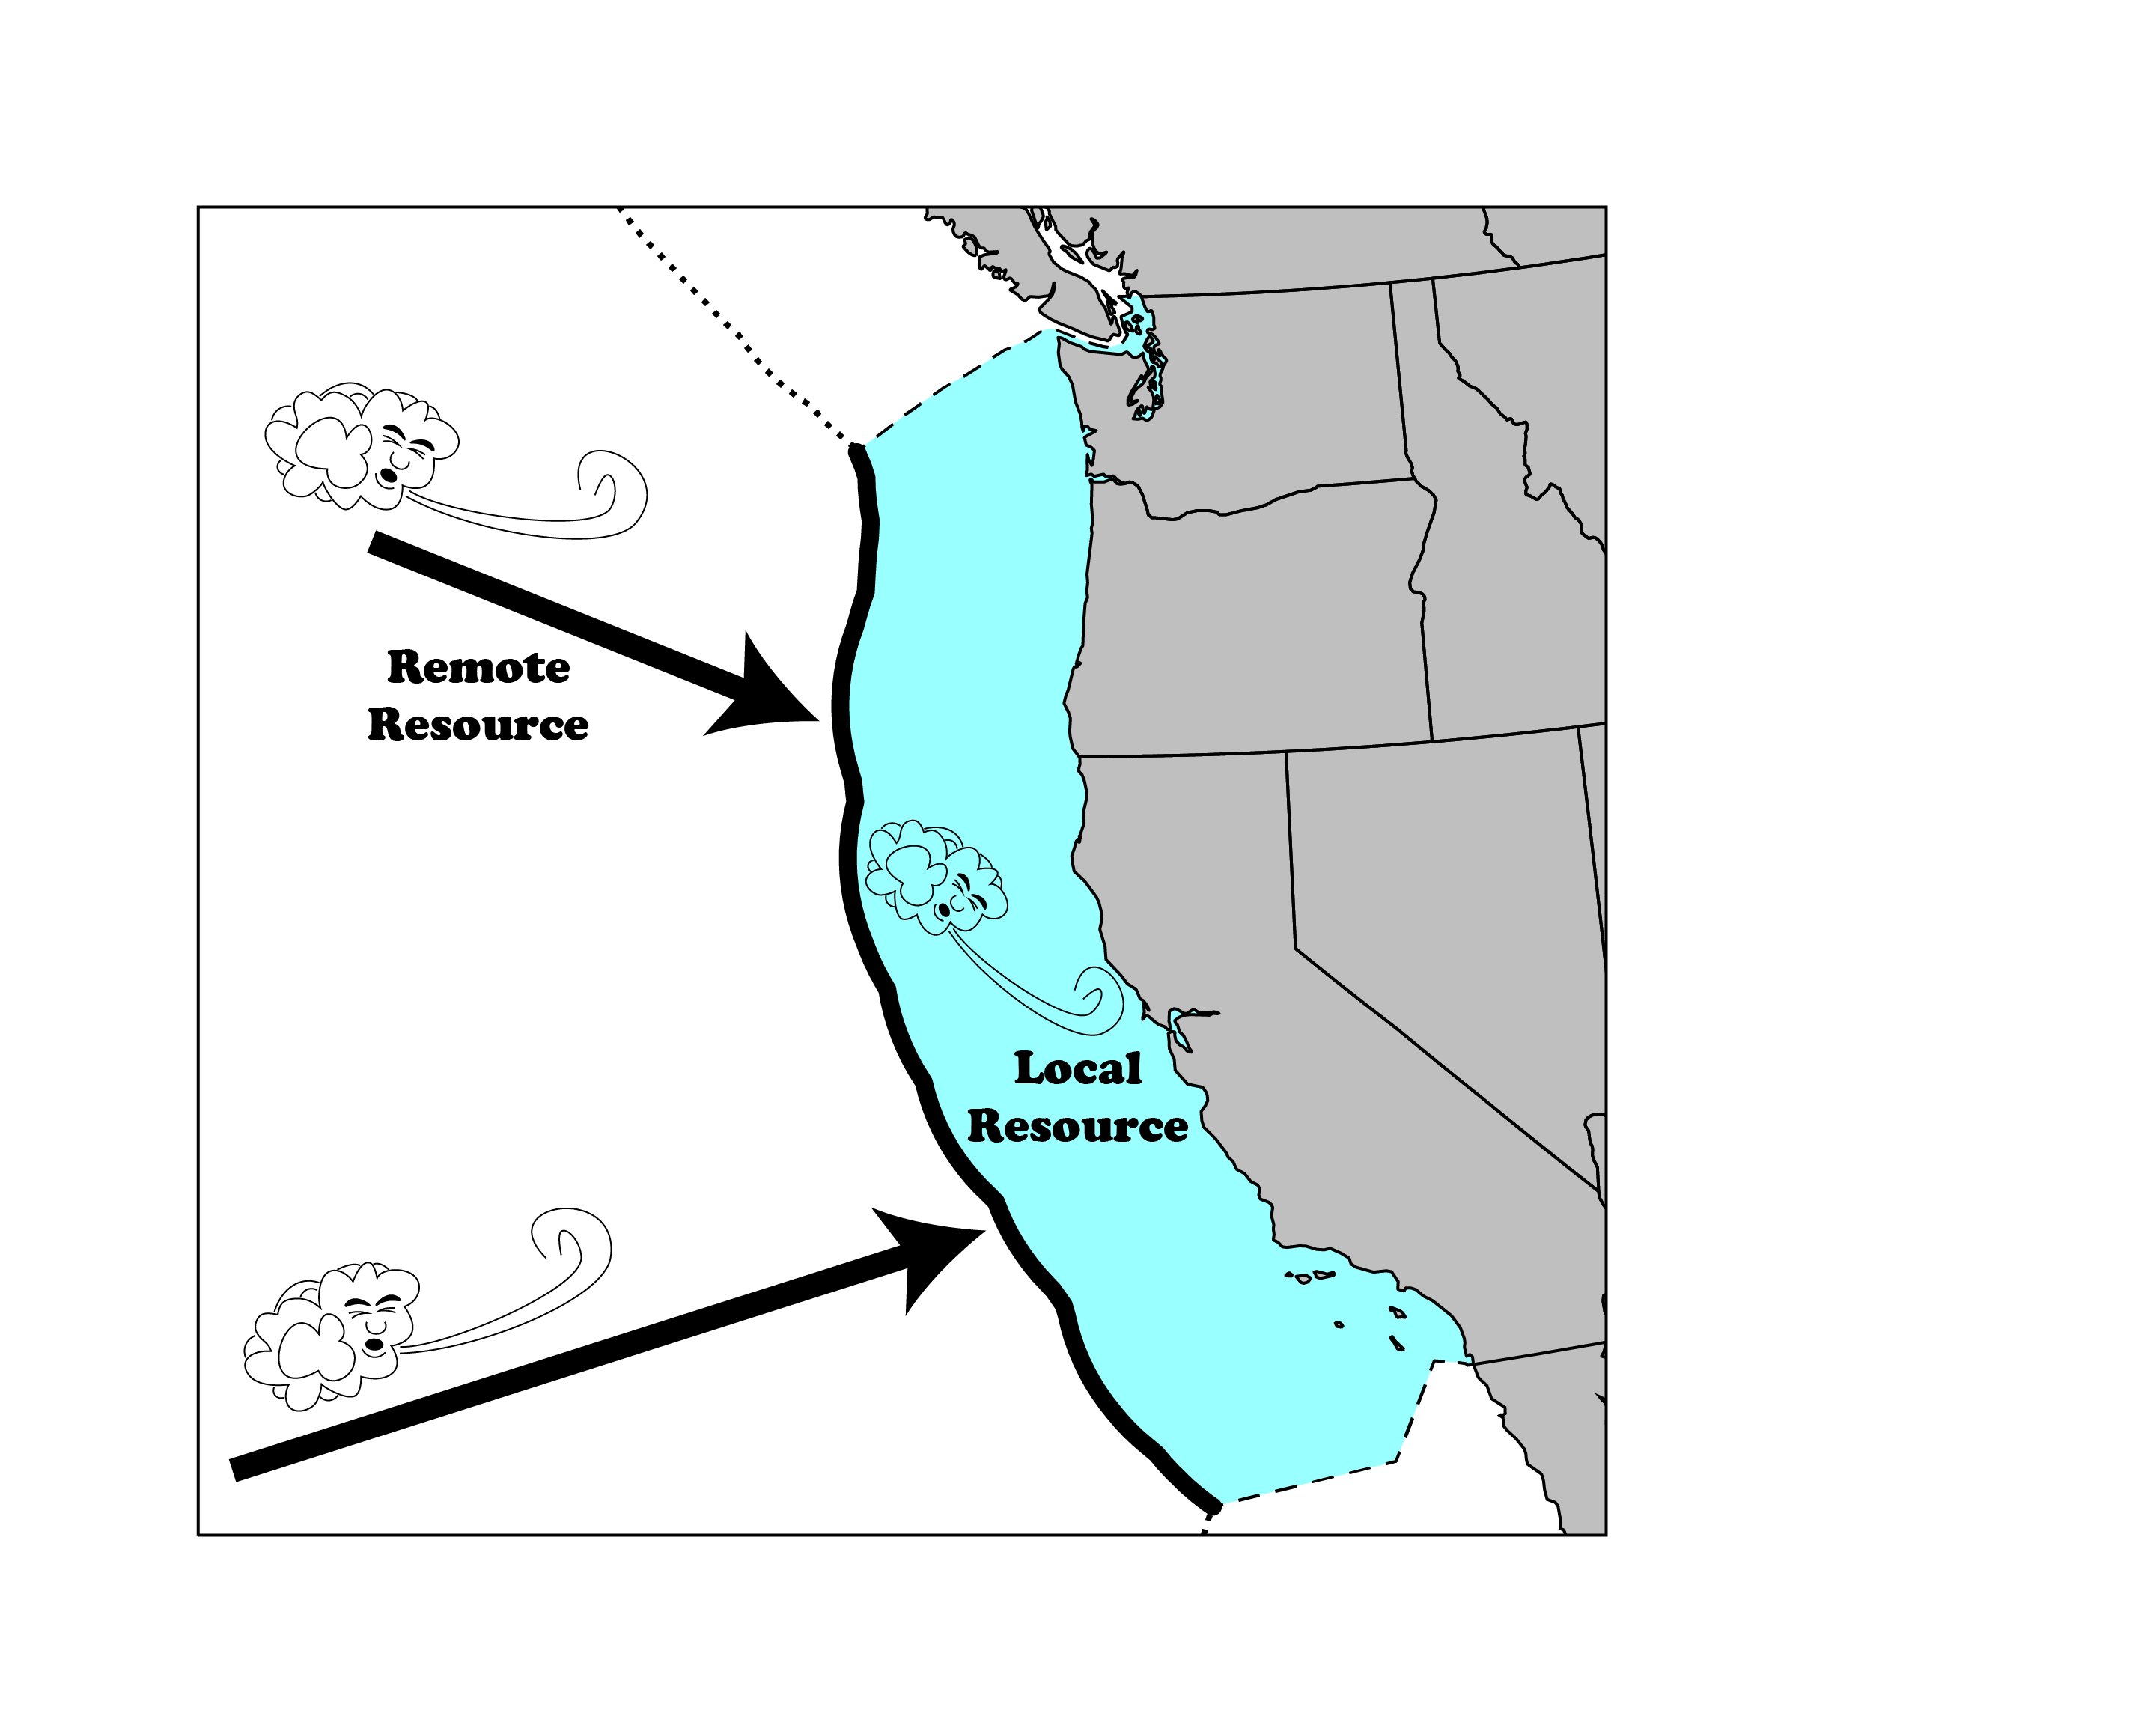
\includegraphics[width=0.9\linewidth]{../diagram/EEZ_contour03_edit01.png}
  \caption{A diagram depicting the U.S. West Coast’s ‘remote’ (arrows) and ‘local’ (cyan region) resource.}
  \label{fig:diagram:west-eez}
\end{figure}

A secondary objective of this work is to provide a refined estimate of the U.S. wave resource based on this new method, and new model results. A tertiary objective is to provide guidance that helps address limitations in site assessment, which we hope will eventually lead to a unified methodology for site and regional wave resource assessment.

These objectives are accomplished by first discussing the details of regional assessments (section 2), and then presenting our proposed approach (section 3). In section 4, we present the results of this approach applied to each region of the U.S. coastline in comparison to alternate methods that have been used. Section 5 provides a detailed discussion of the results, including a justification for the proposed approach, and a summary of how the proposed approach can be applied in different scenarios. We conclude with a summary of results, the proposed methodology, and a view toward how to unify wave energy site and resource assessment
% Need to define `theoretical resource assessment'

This paper has two primary objectives: 1) to define a new methodology for quantifying theoretical wave resource that addresses critiques of previous approaches that can be applied at any scale, and 2) to apply that method to all U.S. regions to obtain an updated assessment of the nation's wave energy potential (theoretical resource).

% Need to define:
% - "WEC"
% - "EPRI2011" (+ EPRI2004?)
% - Ref PBE here? ... Part of motivation for getting this right?


\subsection{Discussion re PBE}
% Need to review the PBE reports.

\begin{itemize}
\item Coastal resiliency?
\item What about mitigating coastal erosion? ... {\it Issue here: WEC devices shut-down during the big events that cause erosion?! ... but what about future tech?!}
\item What about marine shipping? ... wave-powered boat!? WaveGlider? ... Does this belong elsewhere?
\end{itemize}

The methodology developed here has been guided by the successes and limitations of previous works. In particular, several previous works have accurately quantified the remote resource, while others have utilized approaches that have been criticized for 'double counting'. Those works have shot back that, "sure, but you're not accounting for local winds".
\note{How to say this more tactfully?}


%%% Local Variables:
%%% TeX-master: "wave_res"
%%% End:
